\section{Dise\~no de primers para PCR} \label{dna2}

La reacci\'{o}n en cadena de la polimerasa 
(\htmladdnormallink{PCR}{http://es.wikipedia.org/wiki/Reacci\%C3\%B3n_en_cadena_de_la_polimerasa})
es una metodolog\'{i}a est\'{a}ndar en cualquier laboratorio de biolog\'{i}a molecular y consta fundamentalmente
de 3 fases que se repiten un n\'{u}mero de ciclos dentro de un tubo de ensayo que se encuentra en un ba\~{n}o:

\begin{figure}
\begin{center} 
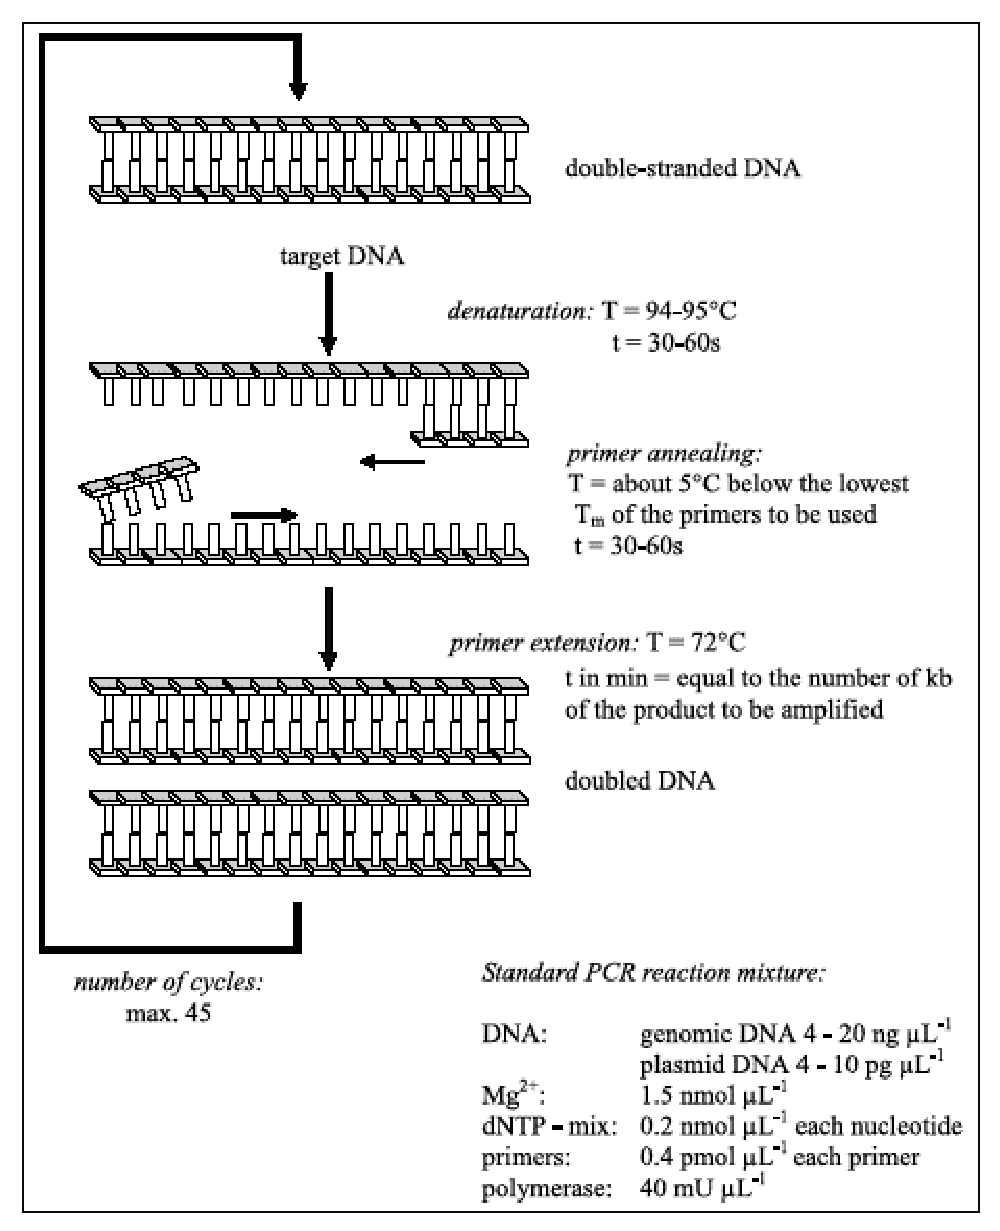
\includegraphics{PCR}
\caption{Diagrama de flujo de una reacci\'{o}n de PCR, 
que consiste en ciclos donde se repiten 3 fases: desnaturalizaci\'{o}n, apareamiento y elongaci\'{o}n.
En la primera el ADN se desnaturaliza separ\'{a}ndose las dos hebras.
En la segunda los cebadores o primers se hibridan con las hebras de ADN en posiciones donde las 
secuencias son complementarias y se forman puentes de H entre bases enfrentadas. 
Es una renaturalizaci\'{o}n parcial que se hace ajustando la temperatura a la secuencia de los cebadores. 
Finalmente, en la tercera etapa se ajusta la temperatura para favorecer la extensi\'{o}n de la nueva hebra
a partir de los cebadores por parte de la polimerasa. 
El tiempo de extensi\'{o}n es proporcional a la longitud del producto de PCR (o amplic\'{o}n) esperado
en funci\'{o}n de los cebadores dise\~{n}ados por el usuario y el genoma en cuesti\'{o}n.
Figura de \cite{Konietzny2003} reproducida con permiso de los autores.}
\label{fig:PCR}
\end{center}
\end{figure}

Para cada aplicaci\'{o}n de la PCR es necesario ajustar las condiciones y el dise\~no de la reacci\'{o}n,
por ejemplo:
\begin{itemize} 
\item la duraci\'{o}n de las fases de apareamiento y elongaci\'{o}n
\item el tipo de cebadores o \italics{primers} empleados y sus temperaturas de fusi\'{o}n $T_{m}$ (ver secci\'{o}n \ref{desnat})
\item el tipo de polimerasa utilizada
\item las cantidad de los reactivos y de ADN molde
\item la longitud del amplic\'{o}n o producto de PCR obtenido
\end{itemize}

En esta secci\'{o}n veremos algunos de los algoritmos habituales para el dise\~no de cebadores, 
que deben cumplir al menos tres condiciones: 

%PCR Nearly Always Works and Design Is Not that Important
%Different Methods for Predicting Hybridization Tm Are Essentially Equivalent in Accuracy
%Designing Forward and Reverse Primers to Have Matching Tm\u2019s Is the Best Strategy to Optimize for PCR
%\u201cPrimer Dimer\u201d Artifacts Are Due to Dimerization of Primers
%A BLAST Search Is the Best Method for Determining the Specificity of a Primer
%At the End of PCR, Amplification Efficiency Is Not Exponential Because the Primers or NTPs Are Exhausted or the Polymerase Looses Activity
%Multiplex PCR Can Succeed by Optimization of Individual PCRs

%Aunque hay variaciones seg\'{u}n el uso, los primers se dise\~nan para cumplir con ciertas 
%\htmladdnormallink{condiciones}{http://www.bioquest.org/bioinformatics/module/cooper/Primer_Design/primer_design.htm}:
%; estas temperaturas suelen ser $T_{a} > 55$, lo 
%que se traduce en valores de GC cercanos al 50\% y longitudes entre 17 y 28 nucle\'{o}tidos

\begin{itemize} \label{reqprimers}
\item Una pareja de cebadores debe tener temperaturas de alineamiento muy cercanas para maximizar el rendimiento, 
lo cual suele traducirse en un contenido en GC similar, entre 50\% y 60\%. 
\item Los primers no deben favorecer horquillas (\italics{hairpins}) ni ser complementarios. 
El siguiente esquema muestra un cebador con una horquilla potencial a la izquierda y un par de cebadores que se aparean a la derecha:
\begin{verbatim}
          5'GGGAAA                    5' GGGAAAATTCCAGGATCTAT 3'
             |||| )                       ||||  ||||
 3' TATCTAGGACCTTA            3' TATCTAGGACCTTAAAAGGG 5'     
\end{verbatim}
\item Tras analizar una gran colecci\'{o}n de primers publicados en la literatura, parece que conviene evitar secuencias 
que terminen en GGG,GGT,ATT,CGA,TAA o TTA \citep{Onodera2007}.
\end{itemize}

Hay muchos programas que pueden ayudar en el dise\~no de primers en la web, como por ejemplo:
\begin{itemize}
\item \htmladdnormallink{primer3}{http://bioinfo.ut.ee/primer3/}
\item \htmladdnormallink{Vector NTI}{http://en.wikipedia.org/wiki/Vector_NTI}
\item \emph{in silico} PCR en \htmladdnormallink{procariotas}{http://insilico.ehu.es/PCR/} 
	y en \htmladdnormallink{animales}{http://genome.ucsc.edu/cgi-bin/hgPcr} 
\end{itemize}

o estos otros para dise\~nar primers degenerados, que permiten reconocer y por tanto amplificar varias secuencias similares
\begin{itemize}
%\item \htmladdnormallink{CODEHOP}{http://blocks.fhcrc.org/codehop.html} (sin mantenimiento)%https://icodehop.cphi.washington.edu/i-codehop-context/Welcome} 
\item \htmladdnormallink{amplicon}{http://amplicon.sourceforge.net/} 
\item \htmladdnormallink{primers4clades}{http://maya.ccg.unam.mx/primers4clades/} (espec\'{i}fico para aplicaciones filogen\'{e}ticas, utiliza CODEHOP)
\end{itemize}

Sin embargo, m\'{a}s all\'{a} del software elegido, es importante saber c\'{o}mo se calculan ciertas propiedades moleculares de los primers,
para poder analizar con criterio los resultados obtenidos. 

Por ejemplo, nos puede interesar calcular la $T_{m}$, 
que es la temperatura a la que la mitad de los primers se han hibridado con el ADN molde, 
o la cantidad de ADN bicatenario a cualquier temperatura, por ejemplo a la temperatura de apareamiento, 
la m\'{a}s cr\'{i}tica, que a menudo se aproxima como $T_{m} - 5$.

Una aproximaci\'{o}n burda es llamada regla de Wallace, que se basa solamente en la secuencia,
donde GC y AT son el n\'{u}mero de nucle\'{o}tidos G/C y A/T en la secuencia del cebador, respectivamente \citep{Santalucia2007}:
\begin{equation}
T_{m} \sim 4GC + 2AT
\end{equation}

Otra alternativa m\'{a}s precisa es la siguiente ecuaci\'{o}n, 
que relaciona exactamente la temperatura con la proporci\'{o}n de ADN bicatenario,
donde $[A]$ es la concentraci\'{o}n de hebras en exceso (los primers), $[B]$ el ADN molde que queremos amplificar,
$\Delta H$ el cambio de entalp\'{i}a, $\Delta S$ el cambio de entrop\'{i}a y $R$ la 
\htmladdnormallink{constante de Boltzmann}{http://en.wikipedia.org/wiki/Boltzmann_constant} (R=1.987 cal/mol K):
\begin{equation}
T_{m} = \frac{1000 \Delta H}{\Delta S + Rln([A]-\frac{[B]}{2})} - 273.15
\end{equation}

%\begin{figure}
%\begin{center} 
%
\includegraphics{TvsC}
%\caption{Curva te\'{o}rica que muestra la dependencia entre temperatura y [ADN hibridado], tomada de \citep{Santalucia2007}.}
%\label{fig:TvsC}
%\end{center}
%\end{figure}

En la pr\'{a}ctica combinamos esta ecuaci\'{o}n con el modelo \italics{Nearest Neighbor} (NN, secci\'{o}n \ref{dna1}), 
usando valores experimentales de entalp\'{i}a y entrop\'{i}a obtenidos para dinucle\'{o}tidos.

Con el objetivo de probar estas recetas el siguiente ejercicio incluye:
\begin{itemize}
\item usar cualquier software que conozcas (o de los citados arriba) para dise\~nar varios primers
\item con ayuda del siguiente c\'{o}digo Python evaluar parejas de primers teniendo en cuenta su $T_{m}$ 
de fusi\'{o}n y su potencial de formaci\'{o}n de horquillas
\item compara las $T_{m}$ obtenidas con las que resultan de aplicar la regla de Wallace
\item prueba a modificar el c\'{o}digo para calcular temperaturas de alineamiento donde la proporci\'{o}n
de primer hibridado sea por ejemplo del 95\%
\verbatiminput{code/prog1.2.py}
\end{itemize}
